\chapter{附录}

\section{命令速查}

\begin{table}[H]
\centering
\small
\begin{tabularx}{\linewidth}{@{}>{\ttfamily\raggedright\arraybackslash}p{6.6cm} L@{}}
\toprule
\hd{命令} & \hd{作用} \\
\midrule
python -m finagent all ... & 样例全流程：财报分析、估值、纠错核查 \\
\rowband
python -m finagent locate --input <PDF> & 定位关键页、单位、扫描页 \\
python -m finagent verify-facts ... & 抽取文件证据校验、双通道比对、勾稽 \\
\rowband
python -m finagent verify-extra ... & 经营数据表逐格校验 \\
python -m finagent verify-sources --sources ... & 外部来源登记校验 \\
\rowband
python -m finagent guard ... & 研报文稿数字护栏 \\
python -m finagent numlock ... & 改写稿数字锁 \\
\rowband
python -m finagent.report\_pipeline build ... & 搭建隔离工作区 \\
python -m finagent.report\_pipeline run / refine ... & 启动五个会话；refine 另加盲评与返工 \\
\rowband
python -m finagent.report\_pipeline status ... & 检查 11 道闸门 \\
python -m finagent.report\_pipeline collect ... & 收回产物 \\
\rowband
python -m finagent.report\_pipeline scorecard ... & 多工作区对比 \\
python -m finagent.evaluation run --workspace ... & 对工作区运行质检 \\
\rowband
python -m finagent.evaluation score ... & 改权重后重算分数 \\
python eval/run\_eval.py & 样例评测（抽取与纠错） \\
\rowband
python -m pytest -q tests & 全部测试 \\
\bottomrule
\end{tabularx}
\end{table}

\section{评分标准 v2 全部条目}

\begin{table}[H]
\centering
\footnotesize
\setlength{\tabcolsep}{4pt}
\begin{tabularx}{\linewidth}{@{}l L r l @{\hspace{14pt}} l L r l@{}}
\toprule
\hd{编号} & \hd{条目} & \hd{分值} & \hd{判定} & \hd{编号} & \hd{条目} & \hd{分值} & \hd{判定} \\
\midrule
L0-01 & 数字护栏 & -- & 程序 & L2-04 & 驱动拆解 & 5 & 盲评 \\
L0-02 & 三表勾稽 & -- & 程序 & L2-05 & 历史业绩归因 & 4 & 盲评 \\
L0-03 & DCF 与三表同口径 & -- & 程序 & L2-06 & 行业与竞争 & 4 & 盲评 \\
L0-04 & 免责声明 & -- & 程序 & L2-07 & 预测假设有依据 & 5 & 盲评 \\
L0-05 & 评级与估值一致 & -- & 程序 & L2-08 & 估值方法与参数 & 3 & 盲评 \\
L1-01 & 抽取校验 & 3 & 程序 & L2-09 & 估值交叉验证 & 4 & 盲评 \\
L1-02 & 分部预测基期闭合 & 3 & 程序 & L2-10 & 情景与敏感性 & 3 & 盲评 \\
L1-03 & 股权价值桥加总 & 4 & 程序 & L2-11 & 风险落到假设 & 4 & 盲评 \\
L1-04 & 每股价值复算 & 3 & 程序 & L2-12 & 跟踪指标与失效条件 & 2 & 盲评 \\
L1-05 & 情景排序 & 2 & 程序 & L3-01 & 故事线连贯 & 4 & 盲评 \\
L1-06 & 敏感性方向 & 2 & 程序 & L3-02 & 事实、推论、观点可区分 & 3 & 盲评 \\
L1-07 & 终值占比 & 2 & 程序 & L3-03 & 结论先行 & 3 & 盲评 \\
L1-08 & 预测与历史衔接 & 2 & 程序 & L3-04 & 无机器腔 & 3 & 盲评 \\
L1-09 & 正文估值与产物一致 & 3 & 程序 & L3-05 & 数字密度 & 2 & 盲评 \\
L1-10 & 外部信息可追溯 & 4 & 程序 & L3-06 & 图表服务论点 & 3 & 盲评 \\
L1-11 & 股价有日期与来源 & 2 & 程序 & L3-07 & 假设与局限透明 & 2 & 盲评 \\
L1-12 & 复核改写过数字锁 & 3 & 程序 & N-01 & 无来源的外部数据 & $-8$ & 盲评 \\
L1-13 & 人工复核清单 & 2 & 程序 & N-02 & 数字前后矛盾 & $-8$ & 程序 \\
L2-01 & 核心结论 & 4 & 盲评 & N-03 & 聚合数构成描述错误 & $-6$ & 盲评 \\
L2-02 & 预期差 & 4 & 盲评 & N-04 & 结论前后冲突 & $-8$ & 盲评 \\
L2-03 & 商业模式 & 3 & 盲评 & & & & \\
\bottomrule
\end{tabularx}
\end{table}

\section{术语}

\begin{description}[leftmargin=0pt,labelsep=0.6em,font=\heiti\bfseries\color{ink},itemsep=3pt]
  \item[真值表] 经证据校验与双通道核对后的财务数据表，“指标 × 期间”，每格带数值、单位、出处与取得方式；估值、纠错与研报写作的唯一数据来源。
  \item[双通道] 模型通道（分析师会话读 PDF 抄数）与规则通道（程序解析表格）独立取数、互相核对。
  \item[证据校验] 在模型所写页码的原文中按数字边界查找所抄数字，找不到即拒收。
  \item[勾稽] 报表之间、科目之间应当成立的等式，如资产 = 负债 + 所有者权益。
  \item[展示精度容差（$\halfulp$）] 研报数字最后一位的一半，如“58.62 亿元”的容差为 0.005 亿元。
  \item[数字护栏（guard）] 检查文稿中每个数字的出处、指标期间绑定、外部数字编号与前后一致性的程序。
  \item[数字锁（numlock）] 要求改写稿的数字与来源编号是初稿子集的程序。
  \item[闸门] 每个阶段结束后由程序判断是否完成的条件，前序不过则后续一律不过。
  \item[盲评] 在只含交付物的目录中、看不到生成过程和分值的模型评审。
  \item[FCFF] 企业自由现金流，即税后经营利润加折旧摊销，减资本开支和营运资本增加。
  \item[反向 DCF] 固定其他假设，求解使每股价值等于现价的单个参数值。
\end{description}

\chapter{宁德时代研报全文}
\label{app:catl}

本附录收录系统生成的《宁德时代 2025 年年报点评暨深度研究》全文，原样嵌入，未做任何人工修改。
该报告由 1005 批次流水线生成（2026 年 10 月 5 日），五个会话合计有效时间 63.9 分钟、折合费用 23.59 美元，
全文 42 页（含目录、图表目录、外部资料来源与免责声明），102 个图表；程序评级“买入”，DCF 基准每股价值 359.19 元，参考股价 291.11 元（2026 年 9 月 30 日收盘）。
报告页眉中的 “FinAgent” 是系统早期名称，即本计划书所说的 \sysname{}。

读这份报告时可以留意几处与正文章节的对应：首页“投资要点”与核心数据表中的每个数字都通过了数字护栏（第 7 章）；
深度专题“单位盈利”“储能第二曲线”“去宁化与份额”“全球化”由分析师会话自拟（第 6 章）；
外部数字句末的 S 编号对应报告附录中的外部资料来源，由排版工具从来源登记表自动生成；
盈利预测与估值部分的三情景、敏感性与评级均来自估值引擎的产物（第 5 章）。

\begin{note}[声明]
该报告为系统能力展示，评级与目标价值由程序依据报告中列明的假设计算得出，不构成投资建议。
\end{note}

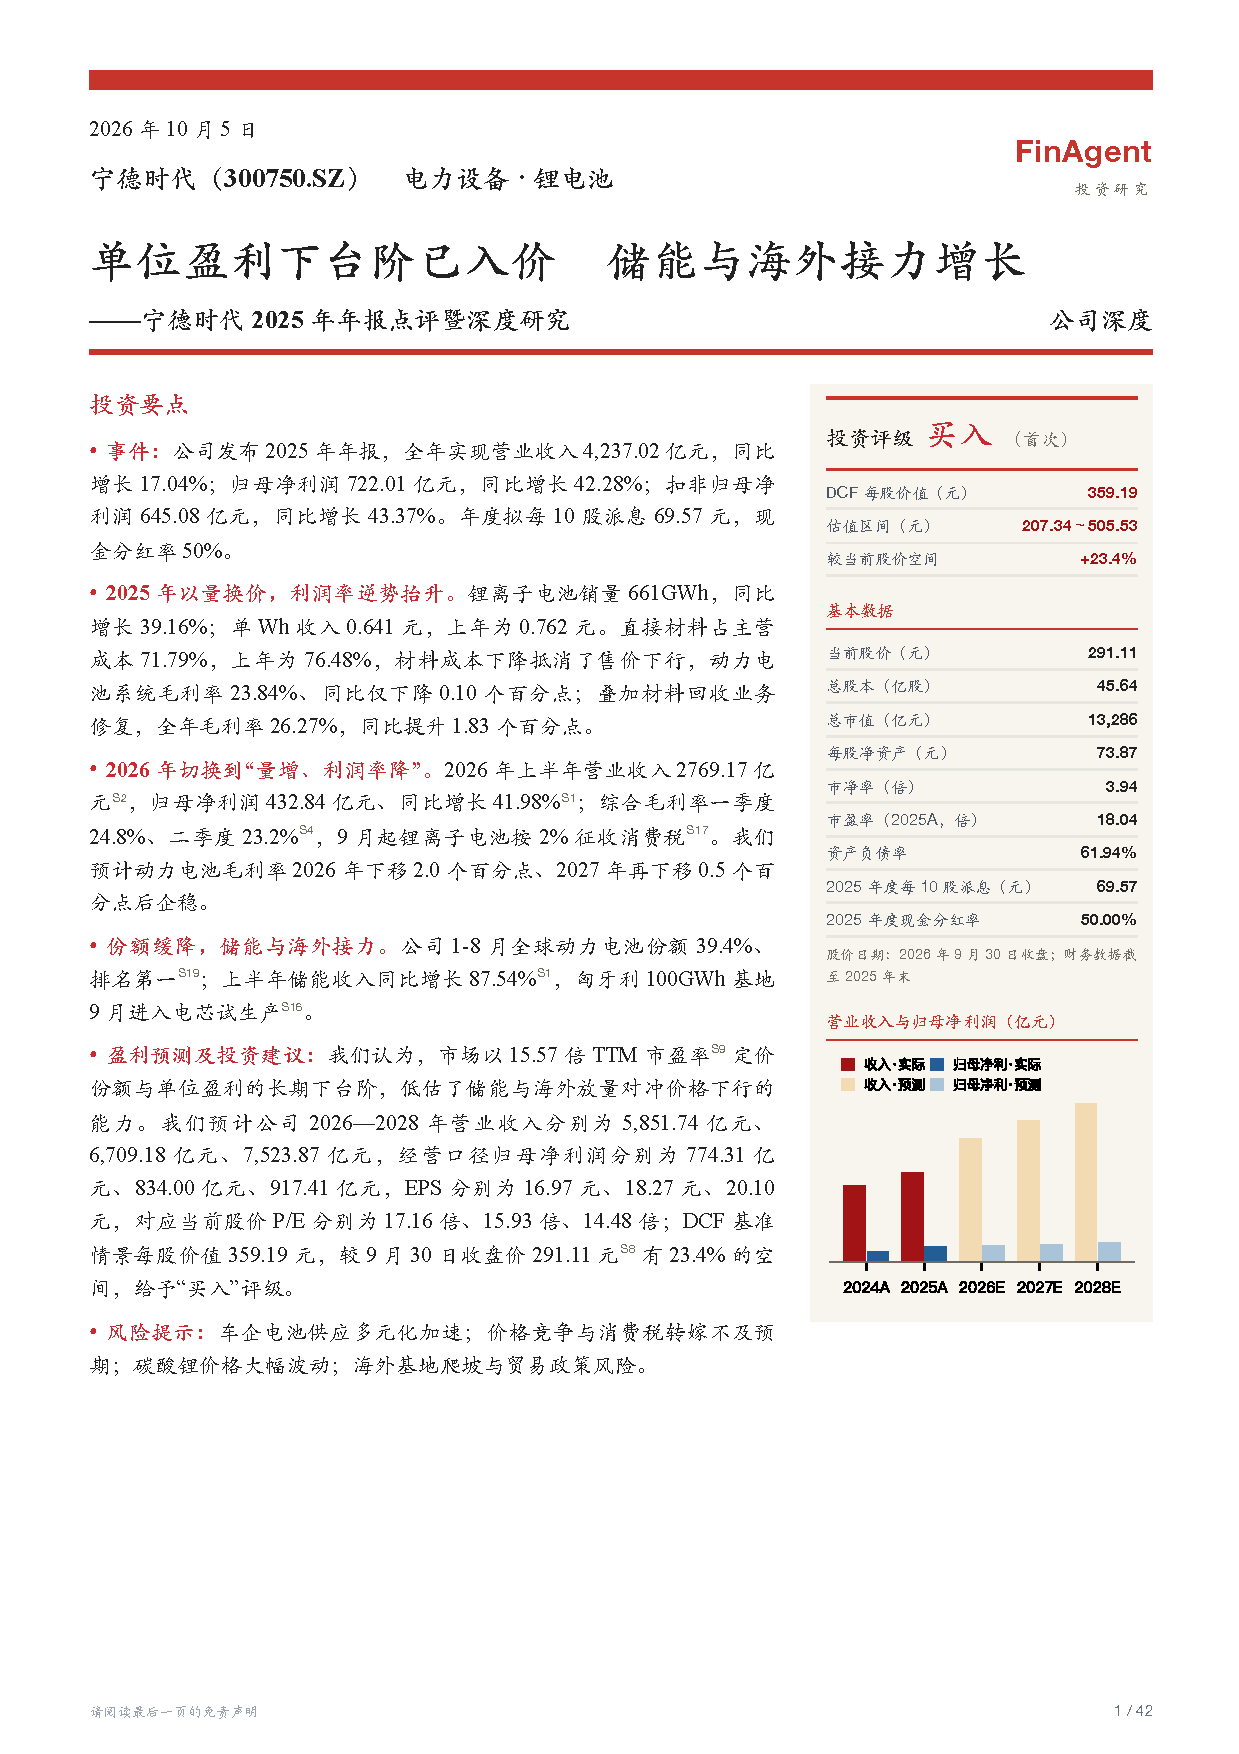
\includepdf[pages=-,scale=0.86,frame,pagecommand={\thispagestyle{fancy}}]{figures/report_catl.pdf}
